\section{Presentation Logic Layer}

%What pages will be present in your project? briefly indicate how your web site will be organized
The presentation layer of FinTrack is organized around a public entry flow, an authenticated area for registered users, and a guest-only calculator area. The main pages are the following:
\begin{itemize}
    \item \textbf{Home page:} The landing page of the application, where users can choose whether to log in, register, or continue as guest.
    \item \textbf{Login page:} A page for returning users, with an email and password form and error feedback for invalid credentials or missing input.
    \item \textbf{Registration page:} A page for new users, with a form for name, surname, email, and password, plus validation and duplicate-email feedback.
    \item \textbf{Dashboard page:} The main authenticated overview page, showing the user's financial summary and the list of wallets currently associated with the account.
    \item \textbf{Forecasting page:} An authenticated analytical page dedicated to scenario-based financial projections generated from the user's transactions, recurring expenses, and PAC plans.
    \item \textbf{PAC page:} A protected page where the user can create, inspect, update, and delete PAC plans.
    \item \textbf{Guest page:} A public calculator area that allows non-registered users to access the loan, compound-interest, and budget calculators together with their related reports.
\end{itemize}

\clearpage
\subsection{Home Page}

The Home page is the public landing page of FinTrack. Its purpose is to present the three main entry points of the system in a simple and immediate way. From this page, the user can choose to authenticate through the Login page, create a new account through the Registration page, or continue without registration by entering the guest calculator area.
\noindent
The page therefore acts as the starting point of the whole navigation flow. It is intentionally lightweight, because its role is not to show financial data but to route the visitor toward the correct experience depending on whether the visitor is already registered or only wants to use the public calculators.

\begin{figure}[H]
    \centering
    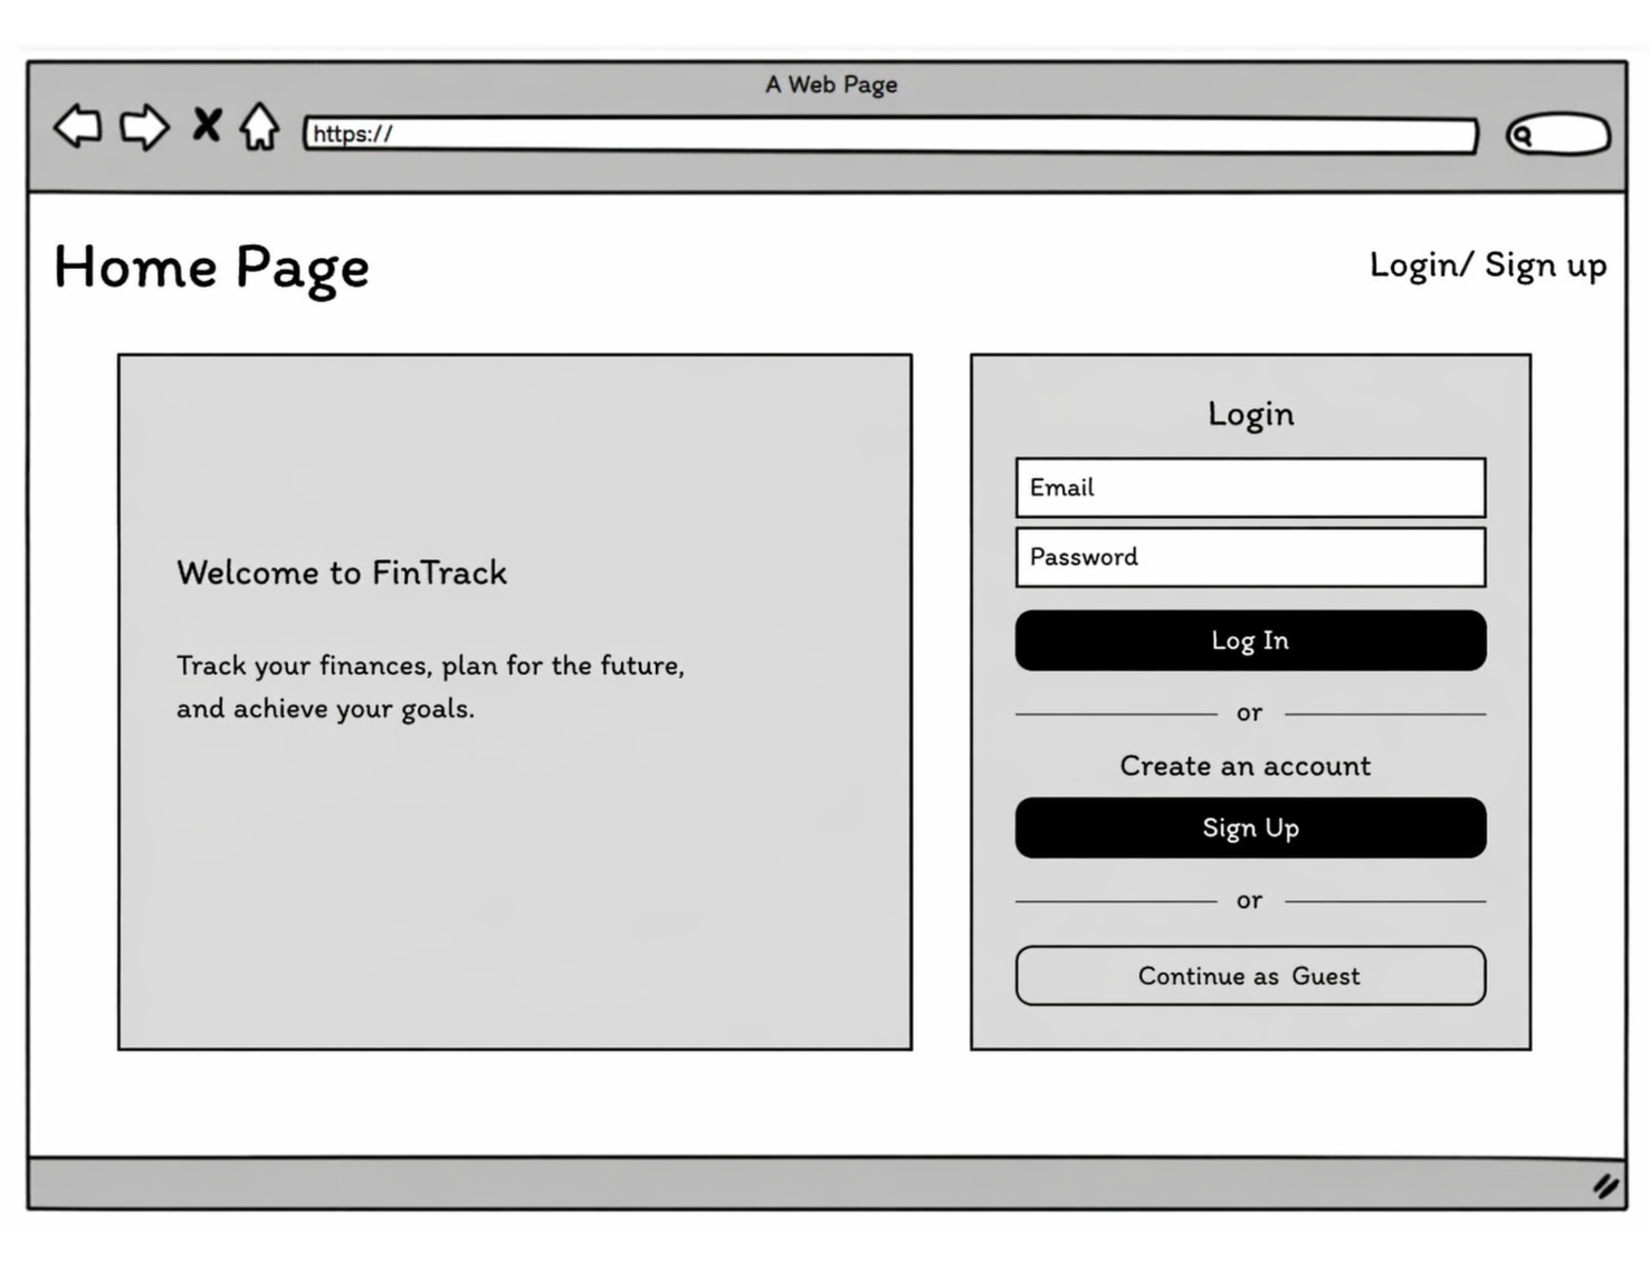
\includegraphics[width=0.8\textwidth]{mockups/home-page.pdf}
    \caption{Home Page}
\end{figure}

\clearpage

\subsection{Login Page}

The Login page is designed for returning users who want to access the protected area of the application. The interface contains a form with two input fields, one for the email address and one for the password. When the form is submitted, the credentials are sent to the authentication servlet, which validates the input and checks whether the account exists and the password is correct.
\noindent
If the authentication succeeds, the user session is initialized and the user is redirected to the Dashboard page. If the input is incomplete or the credentials are invalid, an error message is shown on the same page. A link to the Registration page is also provided so that a visitor without an account can move directly to the sign-up flow.

\begin{figure}[H]
    \centering
    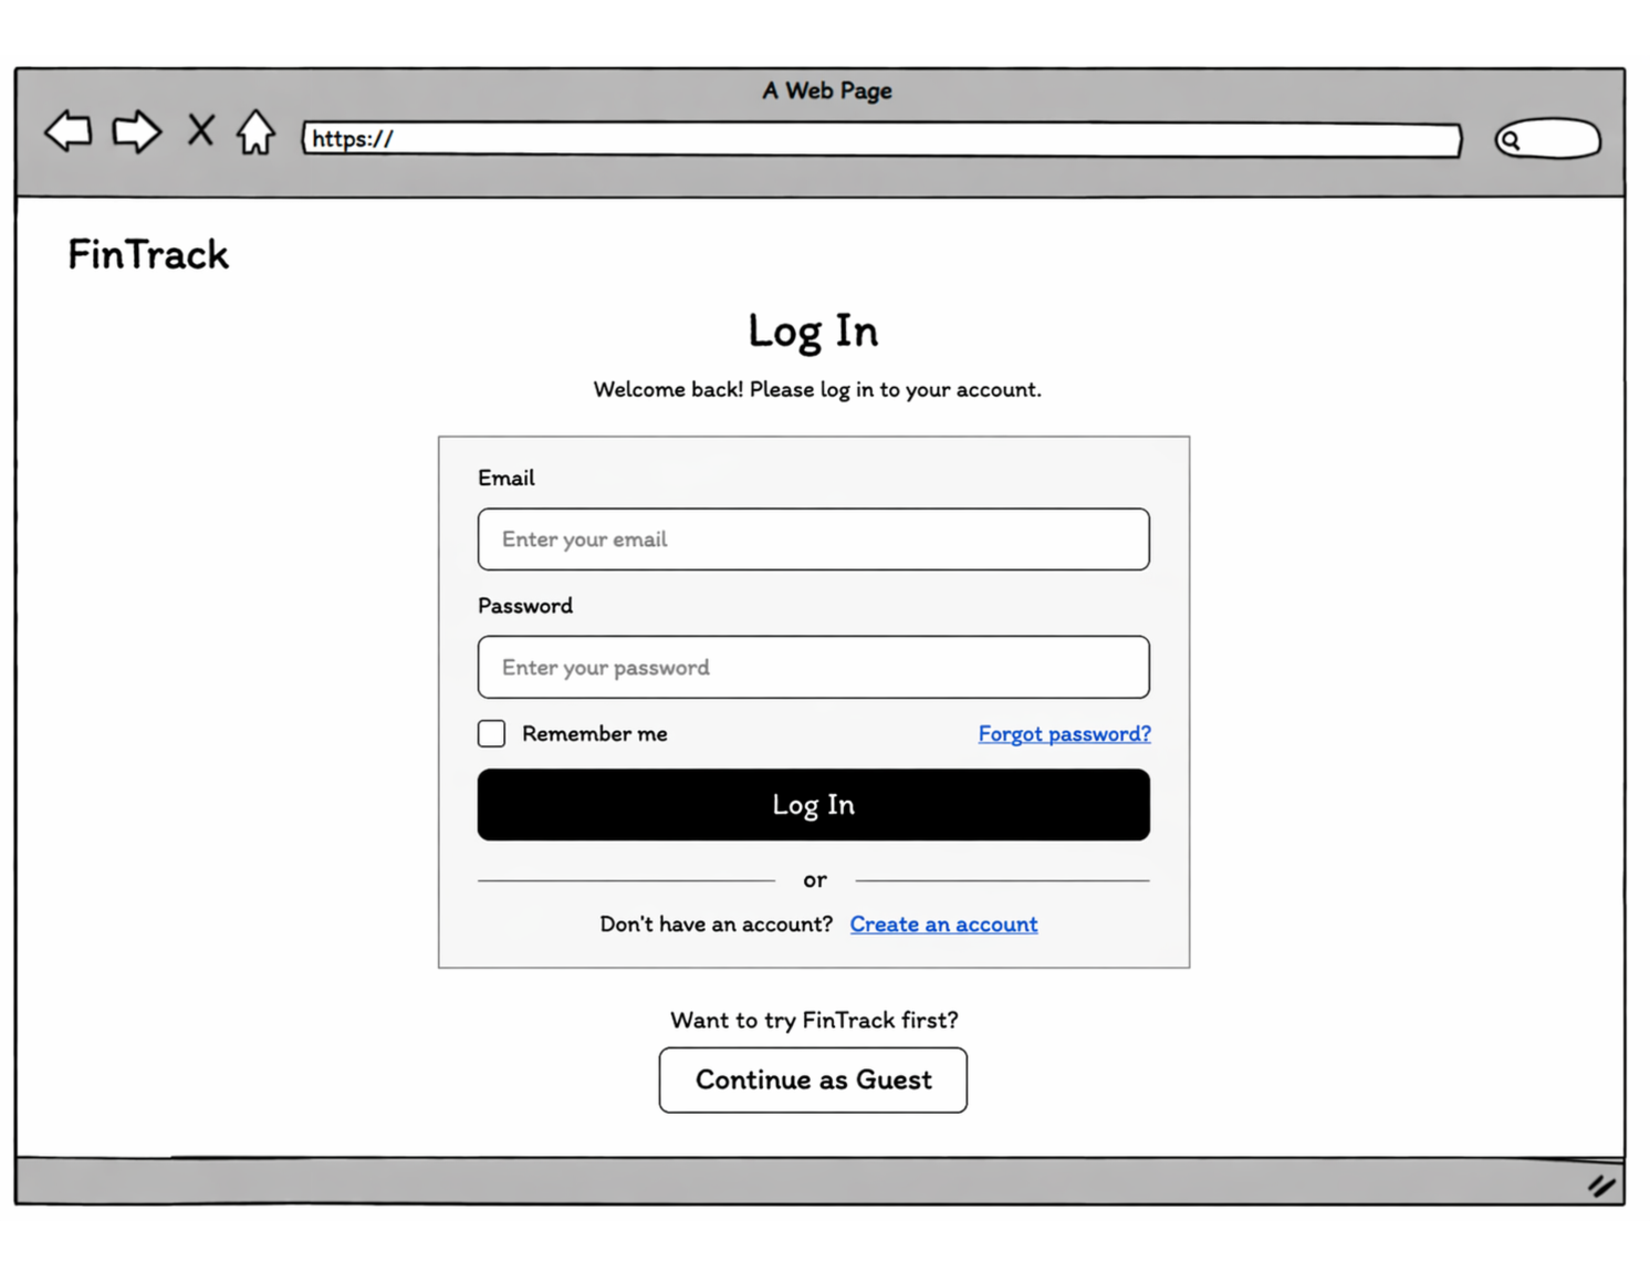
\includegraphics[width=0.8\textwidth]{mockups/login-page.pdf}
    \caption{Login Page}
\end{figure}

\clearpage

\subsection{Registration Page}

The Registration page allows a new user to create a personal FinTrack account. The page contains a form with the fields required by the application logic: name, surname, email, and password. These values are validated before the account is created, so the page must support the display of feedback messages in case one or more fields are missing or the email address is already associated with another account.
\noindent
After a successful registration, the application immediately opens an authenticated session for the new user and redirects the user to the Dashboard page. In this way, the registration flow is integrated with the main personal area of the system without requiring a second login step. The page also includes a link back to the Login page for users who already have an account.

\begin{figure}[H]
    \centering
    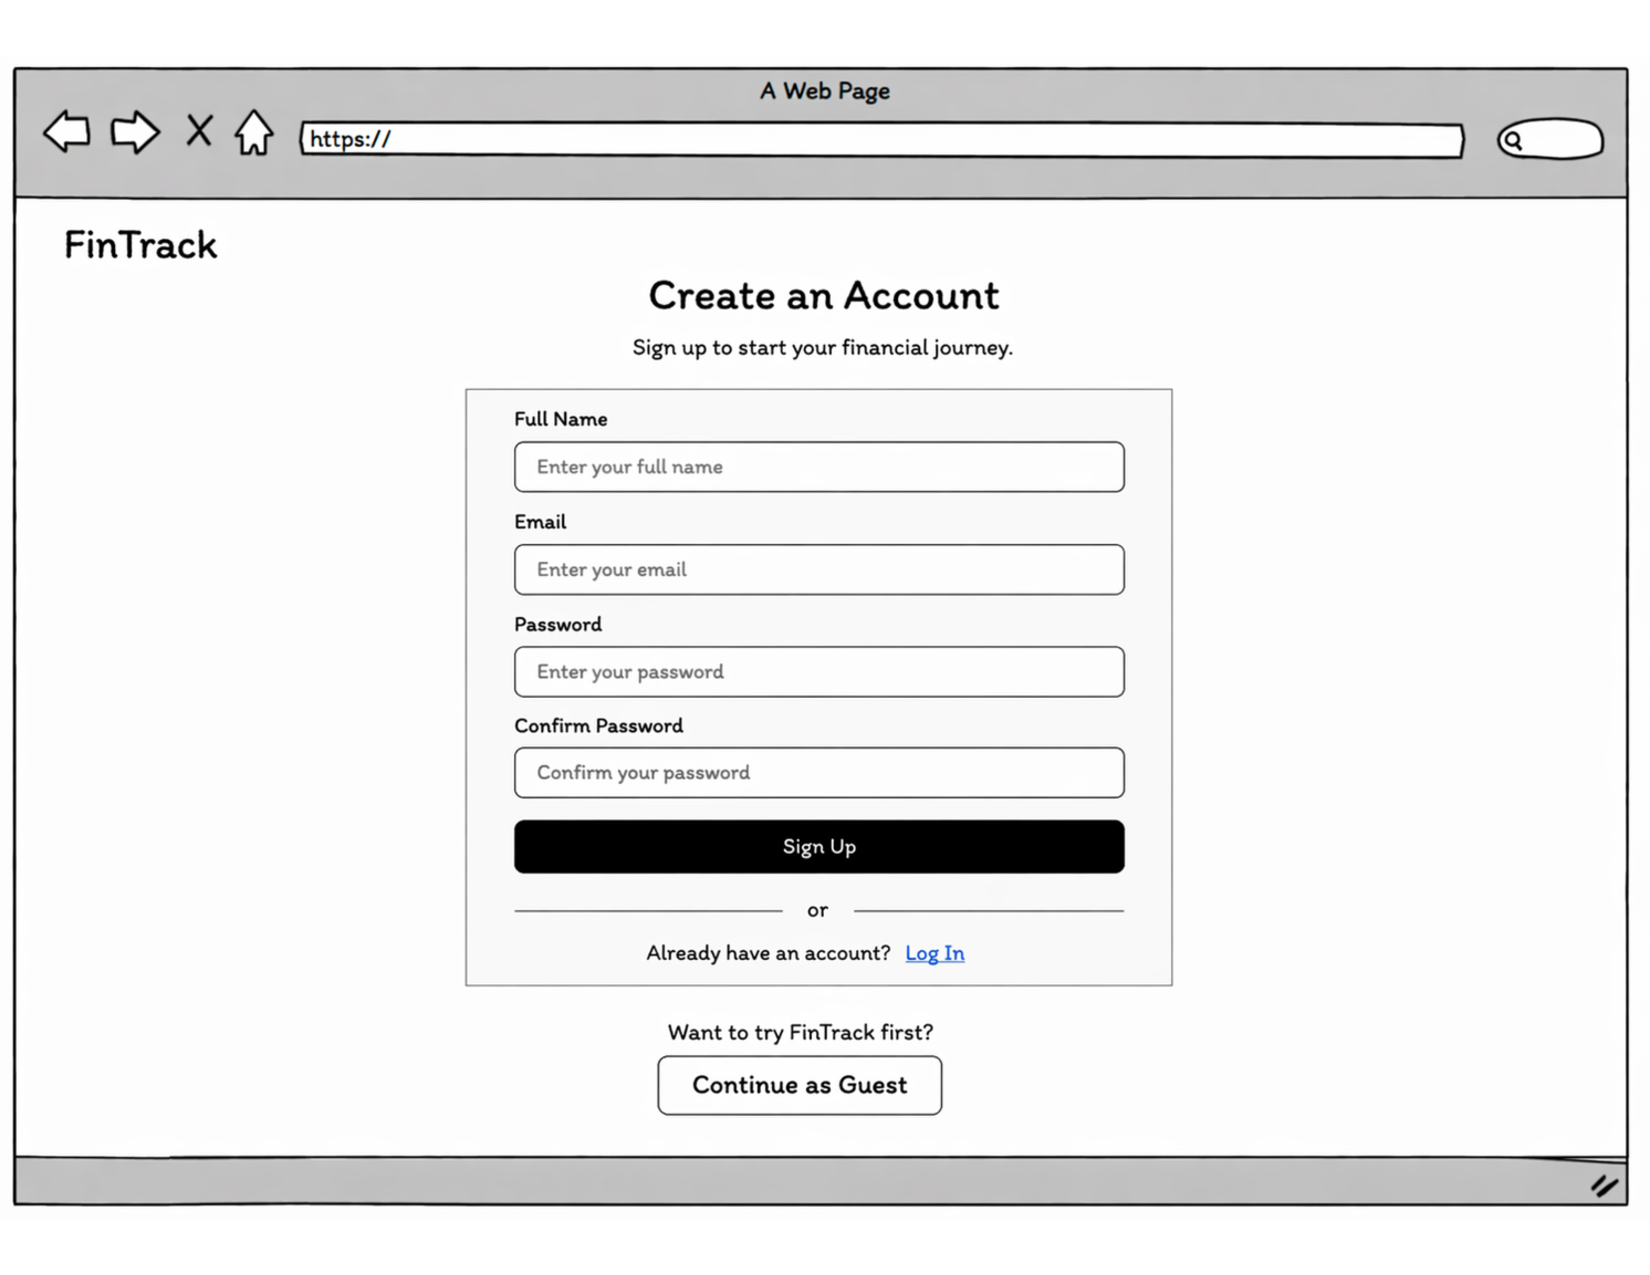
\includegraphics[width=0.8\textwidth]{mockups/registration-page.pdf}
    \caption{Registration Page}
\end{figure}

\clearpage

\subsection{Dashboard Page}

The Dashboard page is the main overview page for authenticated users. At the top, it greets the user by name, confirming that the personal session is active. The page then shows a financial summary containing the main high-level indicators currently produced by the business logic: total equity, year-to-date expenses, and year-to-date savings.
\noindent
Below the summary, the page displays the list of wallets owned by the user. For each wallet, the interface shows the wallet name, wallet type, currency, and current balance. If the user has not created any wallet yet, the page displays a message inviting the user to create the first one. A logout button is also provided so that the user can explicitly terminate the authenticated session.

\begin{figure}[H]
    \centering
    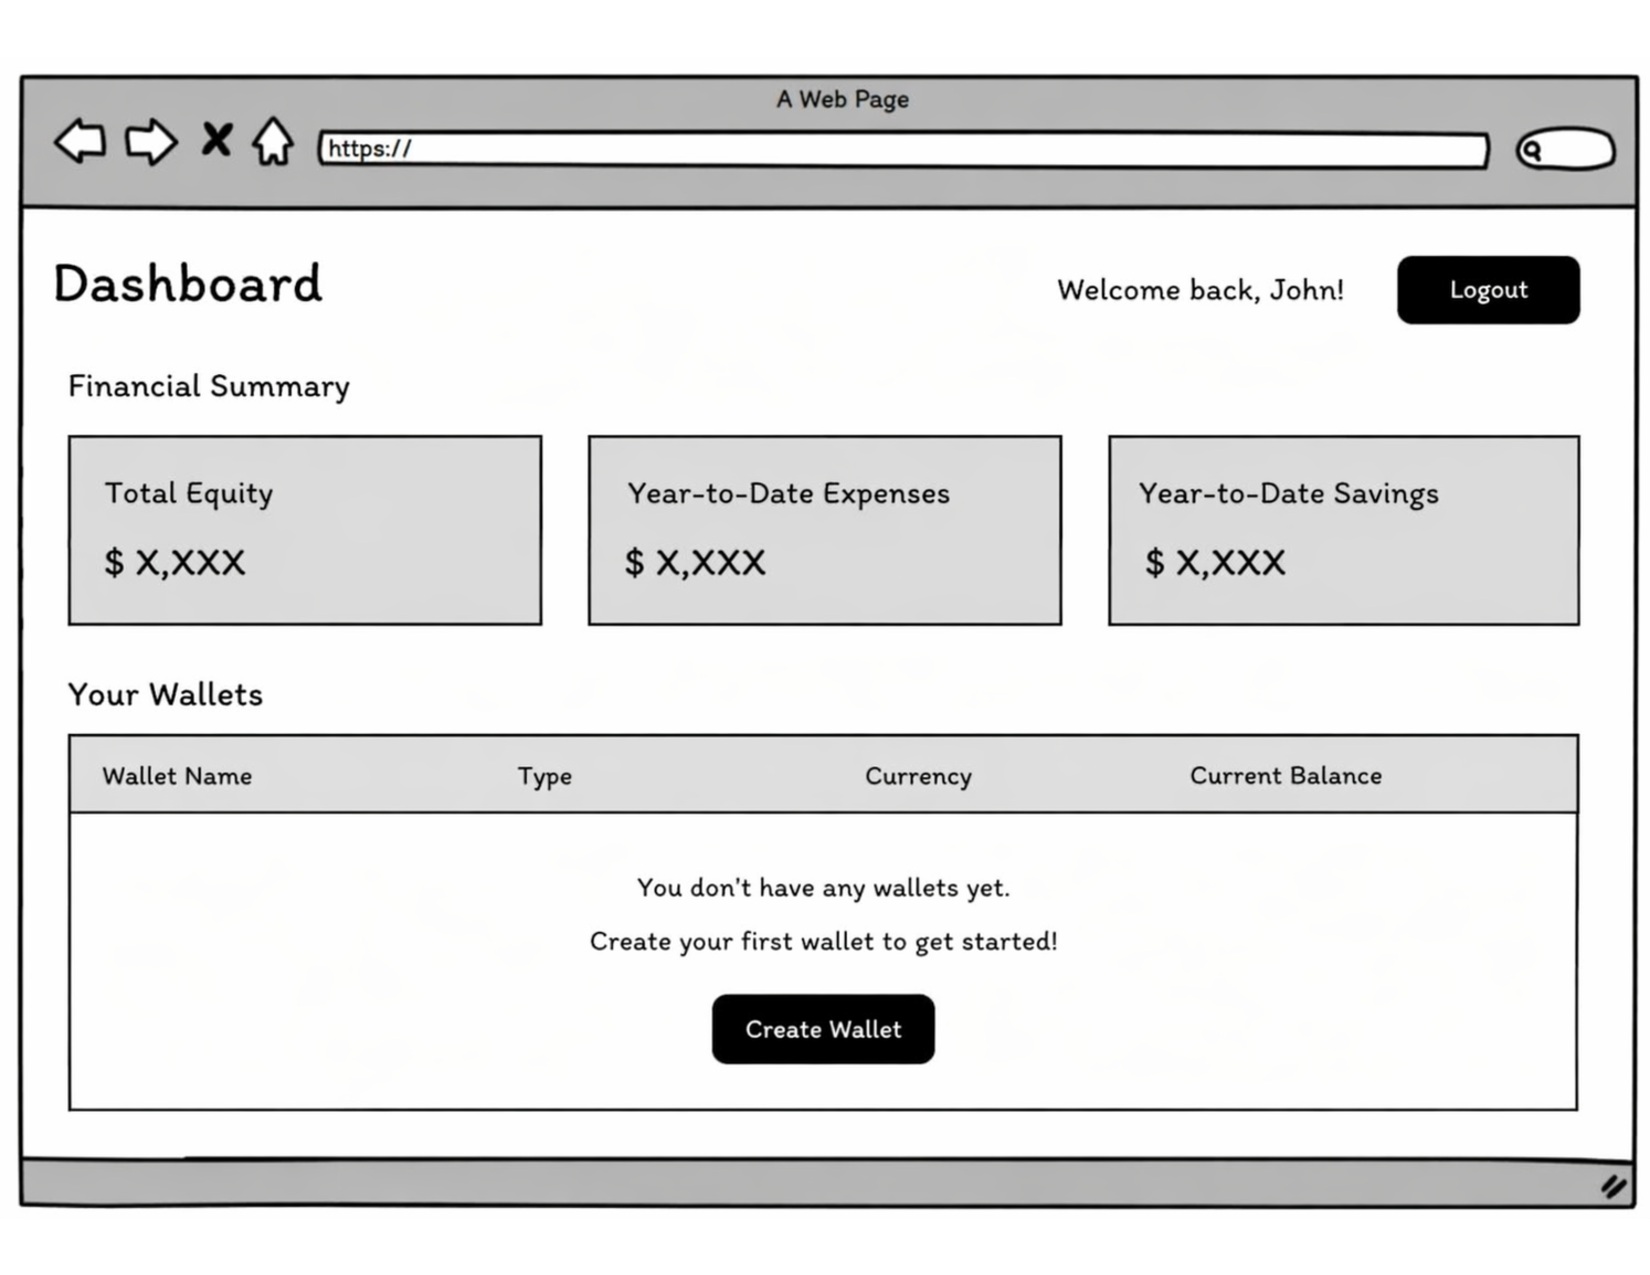
\includegraphics[width=0.8\textwidth]{mockups/dashboard-page.pdf}
    \caption{Dashboard Page}
\end{figure}

\clearpage

\subsection{Forecasting Page}

The Forecasting page is an authenticated analytical page focused on future financial projections. In the current source code, the forecasting functionality is backed by the \texttt{/api/forecast} endpoint, which accepts a scenario and returns a generated projection for the authenticated user. The supported scenarios are \texttt{OPTIMISTIC}, \texttt{CONSERVATIVE}, and \texttt{STRESS\_TEST}.
\noindent
From a presentation point of view, the page is meant to let the user choose one of these scenarios and inspect the generated projection. Each forecast is computed over 24 months and includes, for every month, the estimated income, expense, PAC contribution, net flow, and resulting balance. The page therefore provides a visual and tabular summary of how the user's finances may evolve under different assumptions.

\begin{figure}[H]
    \centering
    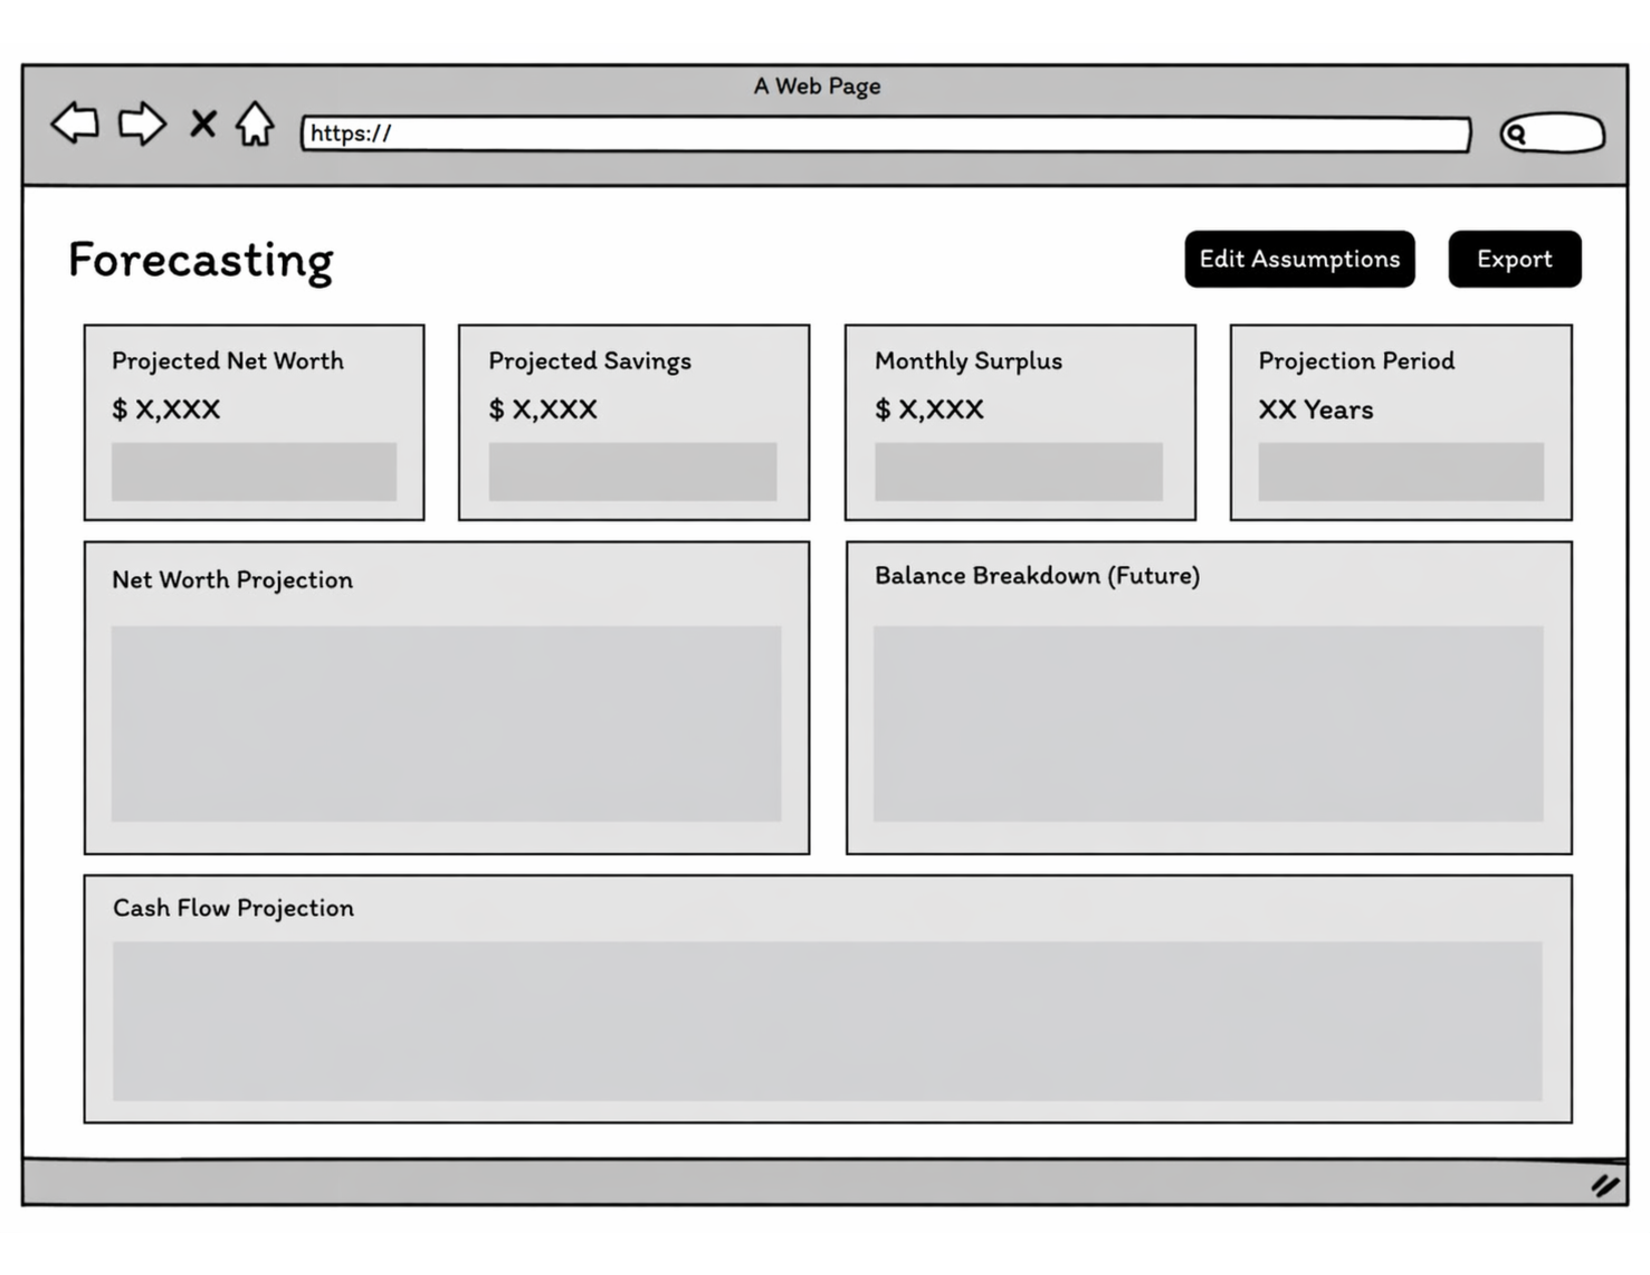
\includegraphics[width=0.8\textwidth]{mockups/forecasting-page.pdf}
    \caption{Forecasting Page}
\end{figure}

\clearpage

\subsection{PAC Page}

The PAC page is a protected management page dedicated to recurring investment plans. According to the application logic, each PAC plan contains an asset name, a monthly contribution amount, a target amount, a start date, and an active flag. The page must therefore allow the user to visualize the list of plans already stored in the system and to perform the main CRUD operations on them.
\noindent
In particular, the interface supports plan creation, modification, and deletion through the dedicated PAC servlets. The page also shows success or error messages after each operation, for example when a plan is created correctly, when validation fails, or when the user attempts an unauthorized action. This page is important because PAC plans are also reused by the forecasting logic as part of the monthly projection.

\begin{figure}[H]
    \centering
    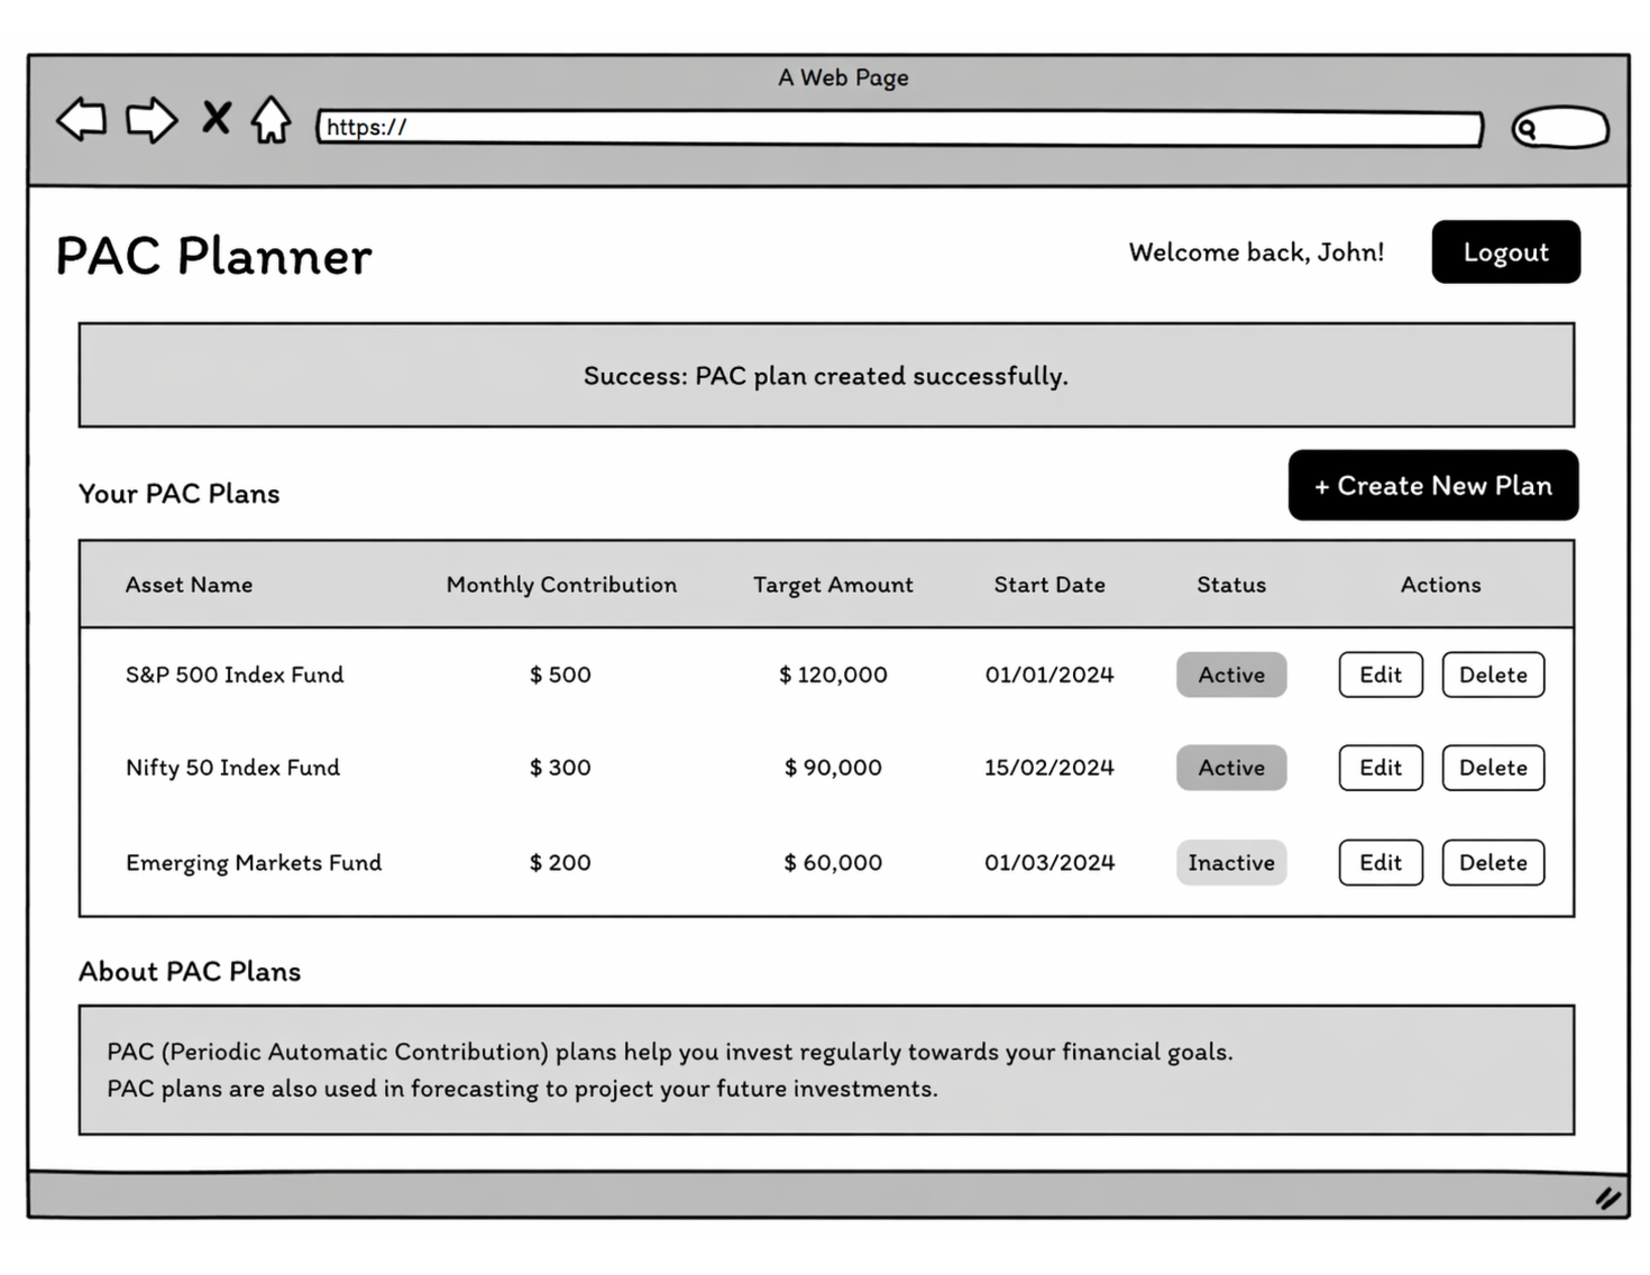
\includegraphics[width=0.8\textwidth]{mockups/pac-page.pdf}
    \caption{PAC Page}
\end{figure}

\clearpage

\subsection{Guest Page}

The Guest page is the public calculator area of FinTrack and is accessible without creating an account. When a user enters this area, the system associates the browser session with a guest token and forwards the request to the calculator page. The interface groups together three independent tools: a loan calculator, a compound-interest calculator, and a budget calculator.
\noindent
The loan calculator asks for principal, annual rate, and duration in months, then produces a report page showing the amortization table month by month. The compound-interest calculator collects the initial capital, monthly contribution, annual rate, and duration in years, then shows the total value reached year by year. The budget calculator lets the user dynamically add and remove income and expense rows, and after submission it generates a report page with total income, total expenses, net balance, and a category-by-category breakdown. The Guest page therefore offers a complete public entry point for trying the financial analysis tools before registration.

\begin{figure}[H]
    \centering
    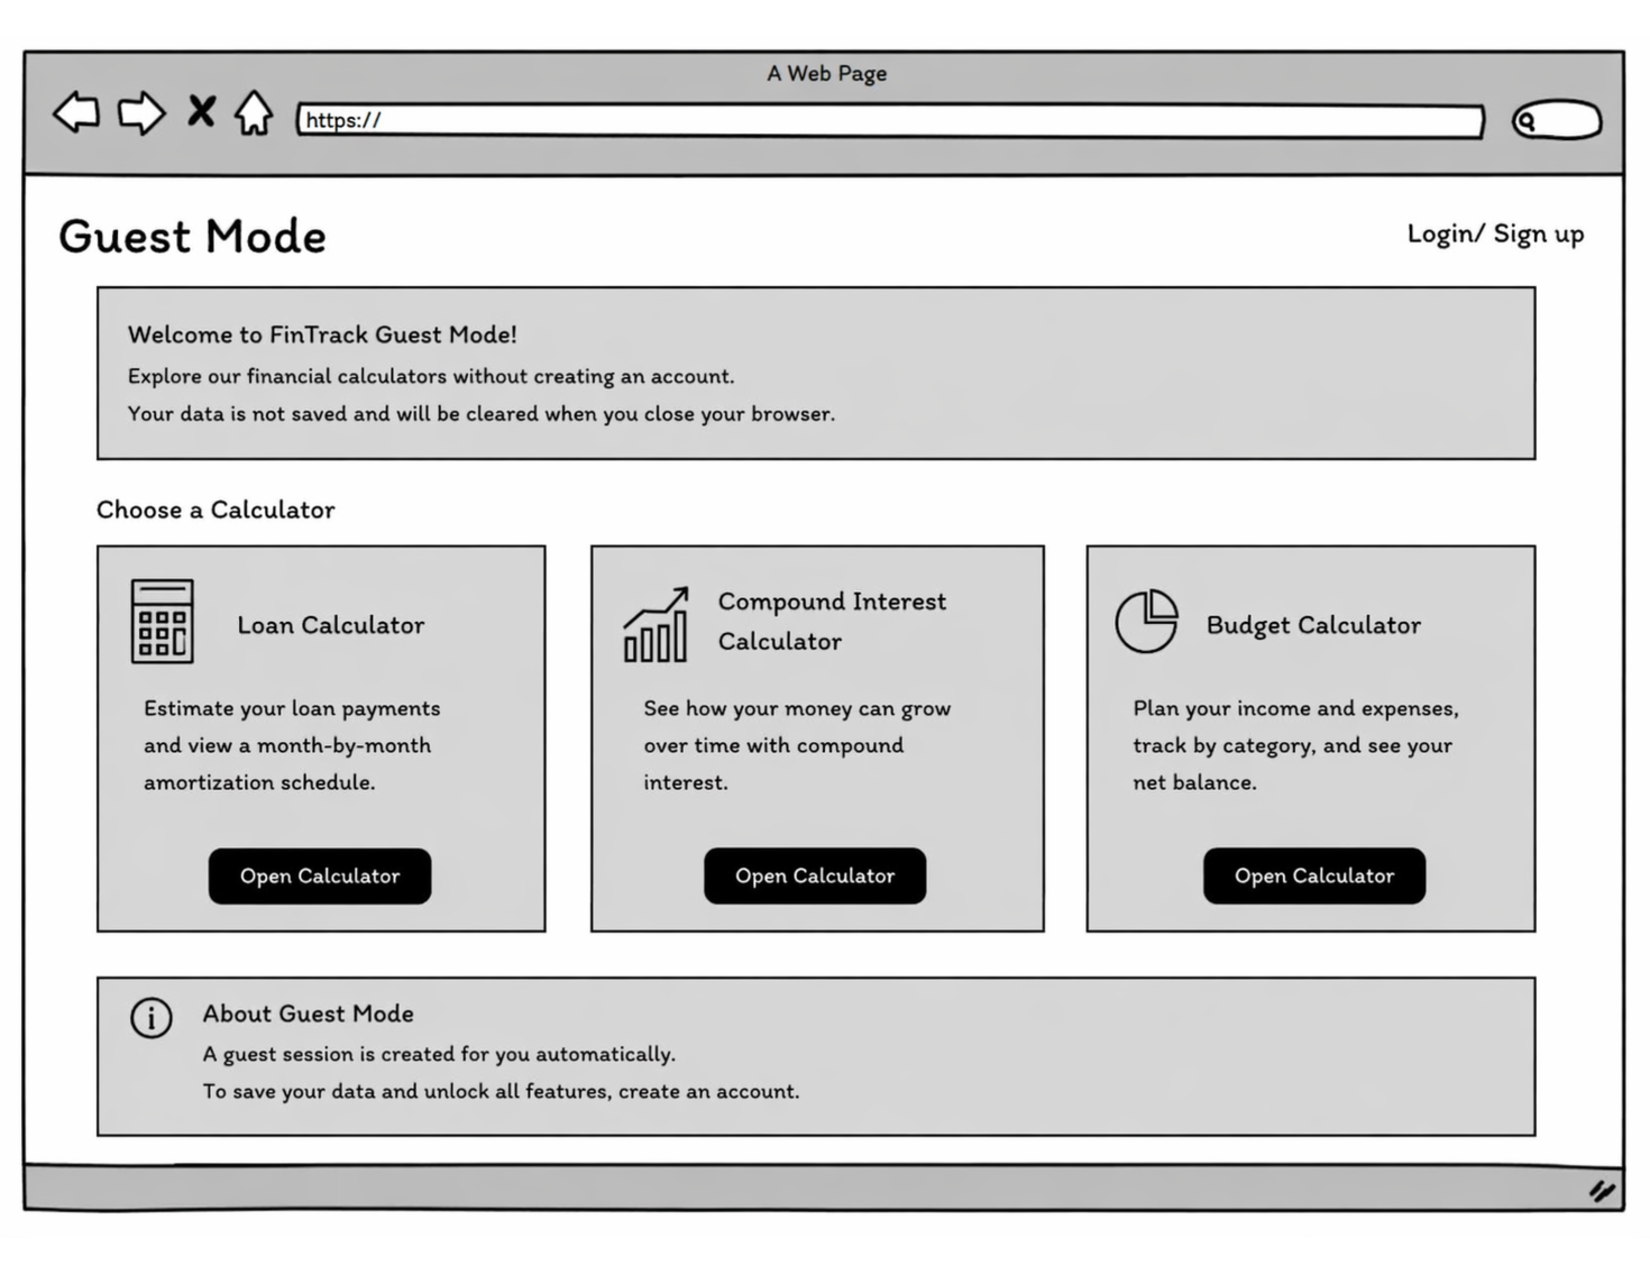
\includegraphics[width=0.8\textwidth]{mockups/guest-page.pdf}
    \caption{Guest Page}
\end{figure}

\clearpage
